\chapter{Light emission statistics in correlated random photonic nanostructures\label{chap8}}

\section{Introduction}

The statistical properties of light transport and emission in disordered media has been a matter of intense research during the last three decades. Although the basis of coherent multiple scattering is a well known subject, the phenomenon itself have much to explore and its far from be clearly understood \cite{wiersma1997localization}. \\
The interest in disordered systems exhibiting certain structural correlations is due to the fact that these systems can share properties of both crystalline and fully disordered systems. For instance, the conductivity of liquid metals \cite{ashcroft1966structure} or the cornea transparency \cite{hart1969light} can be understood in the same footing: a disordered but correlated system can present spectral regions of high transparency for electron or light transport. Also, strongly correlated charged colloids can scatter light in such a way that the transport mean free path presents a strong chromatic dispersion \cite{Rojas_2004}. Even in the absence of practically any long range correlations, the structure of the scatterers itself can be used to modify the light emission and transport properties of a disordered system in such a way that transport parameters \cite{garcia2007photonic, sapienza2007observation}, or even the threshold of a random laser \cite{gottardo2008resonance}, can present resonances which can be tuned in advance. \\
It is clear that the structure surrounding a single emitter can largely alter its emission dynamics \cite{Purcell_1946,hernando2006effect,desousa2014ising}. In the last years, several groups considered such effects in a statistical way suitable for the description of disordered systems \cite{hernando2006effect,gersen2000influencing, vallee2006fluorescence,Froufe_PRA_2007,desousa2014ising}.  In particular, Vallée \textit{et al.} \cite{vallee2006fluorescence} showed that several structural properties near a phase transition can be accessed via fluorescence intensity fluctuations. It has been theoretically proven that near field scattering in random systems alters fluorescence dynamics in such a way that microscopic information about the surroundings of a single emitter can be obtained from lifetime fluctuations or from the shape of the statistical distribution tails \cite{Froufe_PRA_2007,Froufe_2008,caze2010near,Sapienza_2011}. 

In this chapter we compare light scattering and emission statistics for single emitters embedded in a random scattering medium undergoing a phase transition. In chapter (\ref{chap7}) it was shown that, for a finite and strongly confined system, instead of phase coexistence, the system can present a dynamical phase switching behaviour. Surprisingly, the radial distribution function $g\left(r\right)$ among scatterers in the system is essentially indistinguishable for both phases. Here we show that light scattering measurements performed in the phase-switching regime do not result in differences in the scattering cross section of the system. Nevertheless, calculations of the statistical properties of decay rates of single emitters pinned at the center of the medium can be dramatically different for different phases in the switching regime. Also the lifetime statistics can provide a direct signature of a phase switching behaviour where light scattering measurements are blind to such a dynamical regime.\\
In Sec. (\ref{sec:chap8_statment}) we describe the physical system and introduce the model under consideration. Sec. (\ref{sec:chap8_discussions}) is devoted to the presentation of the numerical results and discussion and in Sec. (\ref{sec:chap8_conclusion}) we present the central conclusions of this work.


\begin{figure}[h]
\begin{centering}
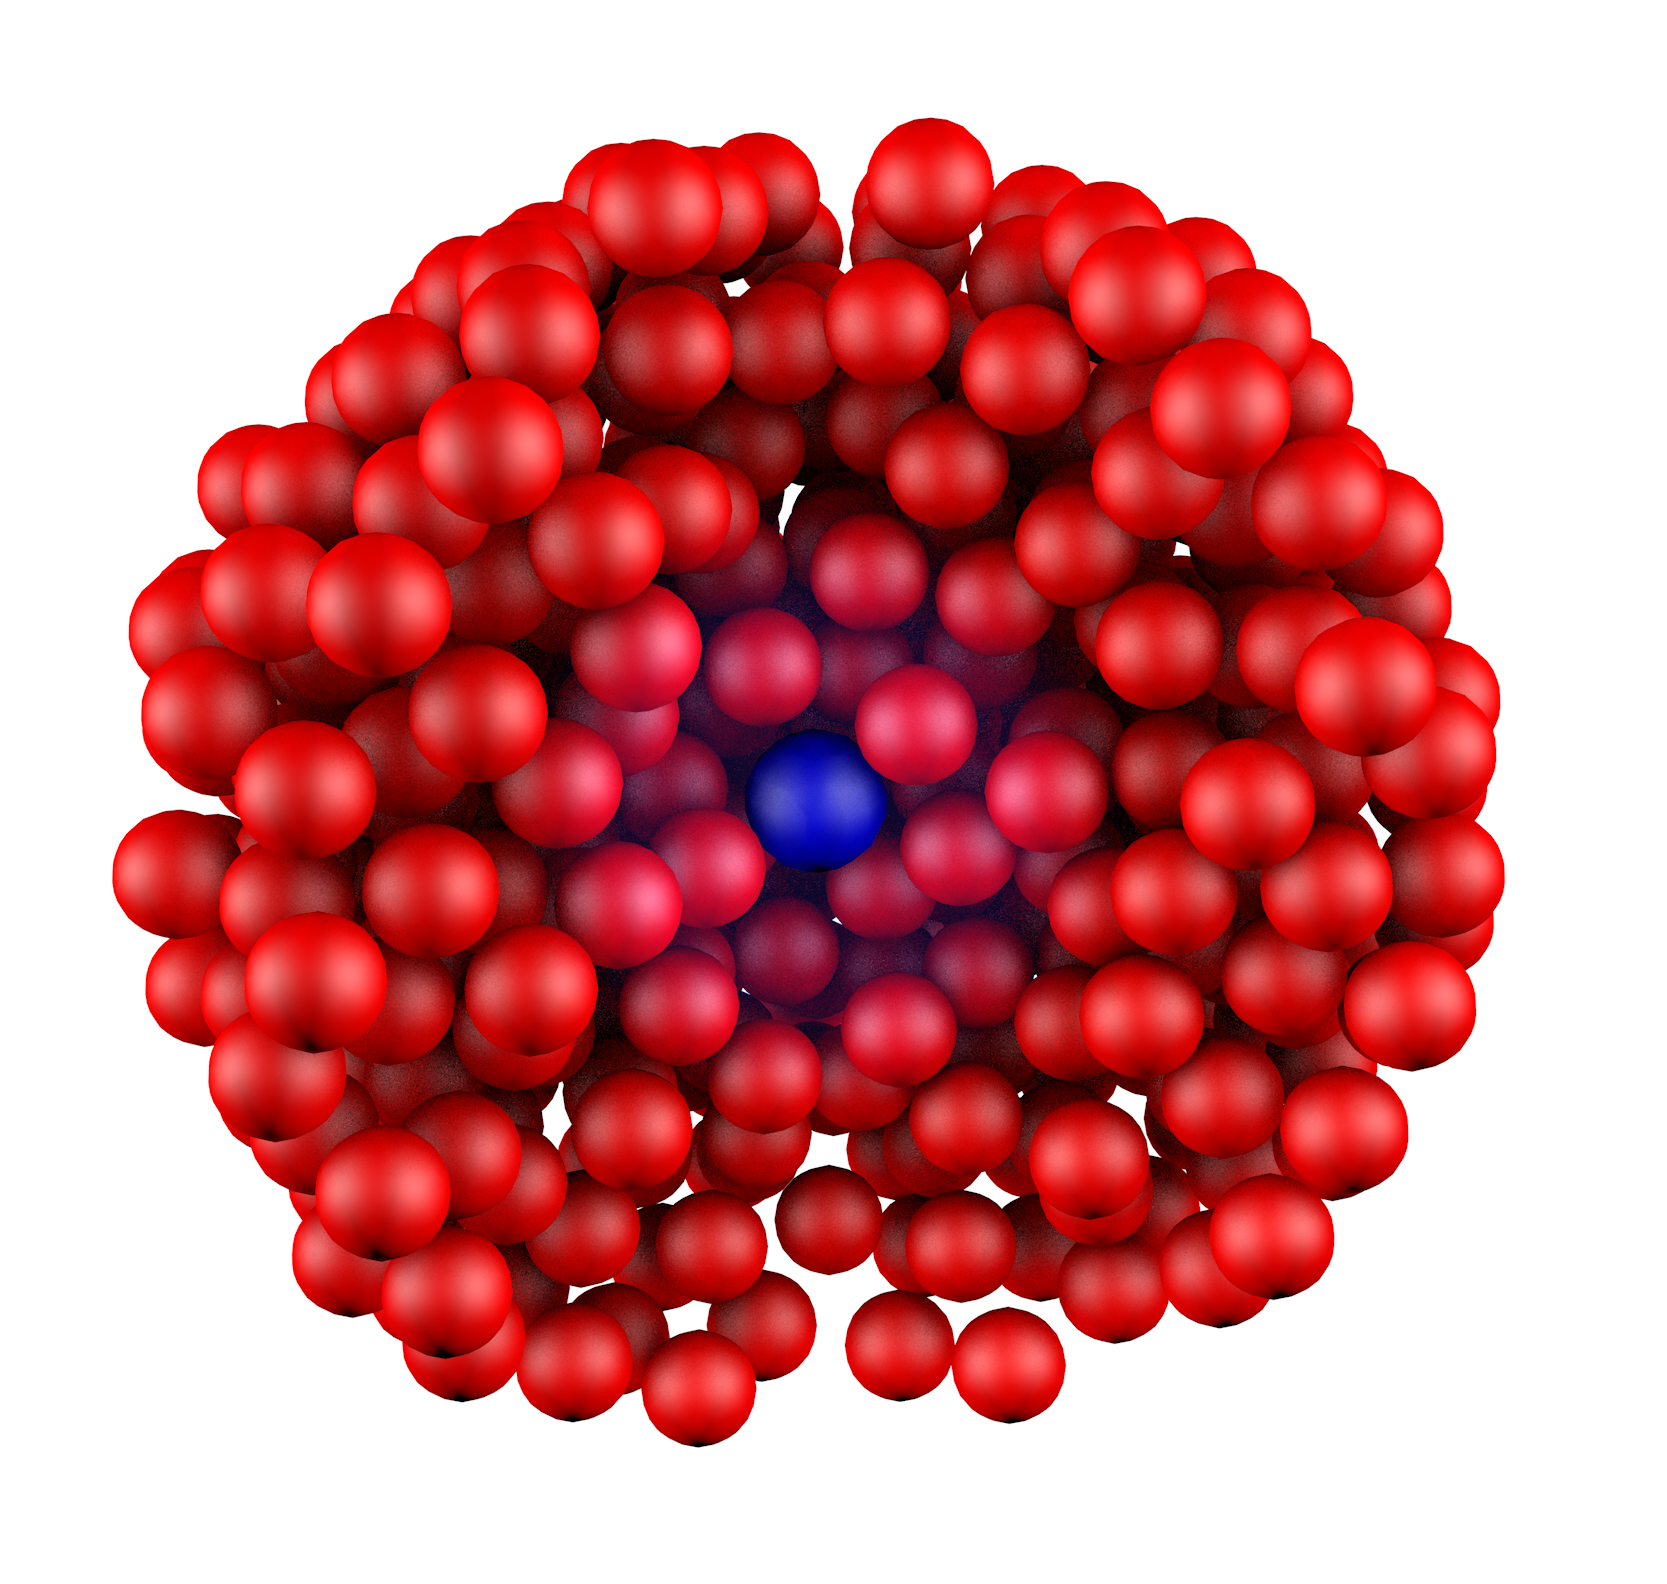
\includegraphics[width=6cm]{chapter_8/figures/sphere_system.png}
\par\end{centering}
\caption{\label{fig:chap8_fig1} Transversal cut of the L-J cluster with $514$ particles. The red spheres represent the point dipole scatterers and the blue sphere in the center represents the point emitter.
}

\end{figure}

\section{Statement of the model\label{sec:chap8_statment}}

The model system under study is a small cluster of $514$ resonant point dipoles interacting through a $\left(12-6\right)$ Lennard-Jones potential. L-J potentials has been extensively studied in the last hundred years. Phase transitions, nucleation dynamics and phase coexistence has been described in great detail in the literature \cite{Hansen:1969tn,Honeycutt:1987,panagiotopoulos1994molecular}.
In chapter (\ref{chap7}) we presented a study of relatively small clusters of particles interacting through L-J potential, in which the systems near a phase transition shows a dynamical phase switching behaviour. In particular, it was demonstrated that in strongly confined clusters with a few hundreds of L-J particles, the system presents an isochoric solid-liquid phase transition at a temperature corresponding to approximately one half of the potential well. Due to the finiteness of the system, the expected specific heat divergence manifests as a peak.\\
In the temperature range corresponding to the phase transition, the system switches in time, in its integrity, between two energetic states that can be associated with solid and liquid phases. In particular, the internal energy clearly shows this behaviour.\\
The pair correlation function obtained in the high and low energy phases is, essentially, indistinguishable. This means that, despite the different dynamical state of each phase, the structural properties of the system, and hence the light scattering properties, should be indistinguishable. We shall consider this point in more detail in following paragraphs.\\
When the self-diffusion coefficients are separately calculated for each phase at constant temperature, we found that there is a three fold variation from solid to liquid phase. Hence, despite the structural indistinguishability among both phases, there is a clear contrast between phases regarding dynamical magnitudes as the internal energy or self-diffusion constants.

The question we want to address is whether or not an optical experiment might show a signature of this phase-switching behaviour.\\
In this chapter we show that indeed this experiment can be realised using fluorescence lifetime statistics measurements but not light scattering.\\
To model the optical response of the interacting particles in the system, we consider each point particle as a point dipole resonant scatterer, similar to those presented in chapter (\ref{chap6}). This model, although not the most general one, covers a wide range of realistic systems that goes from nanoparticles supporting a localised plasmon resonance or cold atom clouds among others. The optical response of the entire system can hence be modelled as an interacting system of point dipoles, a problem that can be readily solved for a system of a few hundred particles in $\sim10^{6}$ different configurations at each temperature by using the coupled dipole method \cite{draine1994discrete}.\\
Using standard Monte Carlo methods, we generate $10^5$ different configurations
of the L-J cluster, each one separated by $10^5$ Monte-Carlo steps. We focus our attention in the temperature of the phase transition, $T\simeq0.53$. We perform light transport and emission calculations for each configuration, evaluating the electromagnetic behaviour of the system as a function of its thermodynamical properties. Results and its subsequent discussion are presented in the next section.

\section{Results and discussion \label{sec:chap8_discussions}}

We start by evaluating the scattering efficiency of a cluster of $515$ L-J particles for different configurations at phase transition temperature. The scattering efficiency is defined by the ratio between the scattering cross section and the geometrical cross section, $Q_{s} = \sigma_{scat}/\sigma_{geom}$.
In Fig. (\ref{fig:fig2}) we present the $Q_s$ (scattering efficiency) sampling at $T \simeq 0.53$. To guide the eye, points corresponding to high and low internal energy are rendered in different colours, where the low energy configuration is rendered in red and the high energy in black. When we integrate the sample in energy, the scattering efficiency histograms are obtained, as shown in Fig.  (\ref{fig:fig2})(a). Differences in $Q_s$ histograms corresponding to high and low energy phases can be hardly distinguished. As expected, we conclude that light scattering experiments would not provide a mean of distinguish among phases in the switching regime.
%We start by evaluating the scattering cross section of a finite crystalline system (FCC lattice) whose first-neighbours distance is the equilibrium distance of the L-J potential $r_{m}$. We obtain a rich pattern in this pseudo-spectrum due to the crystal structure of the system and the resonant character of the scatterers, as can be seen in Fig. (\ref{fig:chap8_crystal_sec}).\\
%
%\begin{figure}[h]
%\begin{centering}
%\includegraphics[width=8cm,angle=-90]{chapter_8/figures/x_sec_vs_k.eps}
%\par\end{centering}
%\caption{\label{fig:chap8_crystal_sec}Scattering cross section spectrum of a crystalline FCC cluster with $515$ L-J particles.}
%\end{figure}
%We take a subset of the whole sam- pling and calculate the scattering cross section of the set of point dipoles. In Fig. 2b ( CREO QUE HAY QUE PRESENTAR LOS PANELES EN ORDEN IN- VERSO: PRIMERO LA NUBE DE PUNTOS Y LUEGO LOS HISTOGRAMAS) we present the energy-Qs (scat- tering efficiency) sampling. To guide the eye, points cor- responding to high and low internal energy are rendered in different colours. Integrating the sampling in energy, we obtain scattering efficiency histograms as shown in Fig. 2a. Differences in Qs histograms corresponding to high and low energy phases can be hardly distinguished. As expected, we conclude the light scattering experiments would not provide a mean of distinguish among phases in the switching regime.
%Nevertheless, not only light scattering in the far field serve as a tool for exploring the structure of a system. Light emission statistics can provide with complementary information.

%We  calculate the energy-$Q_{s}$ (scattering efficiency) for systems at phase transition temperature, $T\simeq 0.53$, with $r_{m}/\lambda = 0.513$, $r_{m}/\lambda=0.466$, $r_{m}/\lambda=0.872$ and $r_{m}/\lambda=0.795$.
%In Fig. (\ref{fig:fig2})(b) we present the results for $r_{m}/\lambda = 0.513$ as example, because for all $r_{m}/\lambda$ the system exhibit a similar behaviour. To guide the eye, points corresponding to high and low internal energy are rendered in different colours. Integrating the sampling in energy, we obtain scattering efficiency histograms as shown in Fig. (\ref{fig:fig2})(a). Differences in $Q_{s}$ histograms corresponding to high and low energy phases can be hardly distinguished. As expected, we conclude the light scattering experiments would not provide a mean of distinguish among phases in the switching regime. \\

\begin{figure}[h]
\begin{centering}
\includegraphics[width=8cm,angle=-90]{chapter_8/figures/2_energy_vs_sec_coex.eps}
\par\end{centering}
\caption{\label{fig:fig2}(a)Energy-scattering efficiency sampling at the switching
region ($T\simeq0.53$, lower panel). (b) We show the
corresponding scattering efficiencies distributions for the upper
energy branch (red distribution) and lower energy branch (black
distribution) corresponding to solid and liquid phases.}
\end{figure}

Nevertheless, not only light scattering in the far field serves as a tool for exploring the structure of a system. Light emission statistics can provide complementary information.\\
In order to assess the possibility of extracting useful information about the structural properties of the system in the switching regime, we consider the statistics of the decay rates of single fluorescent emitters immersed in the structure, as can be seen in the sketch of Fig. (\ref{fig:chap8_fig1}). We start by evaluating the decay rate of a single emitter fixed at the center of the cluster when the particles are perfectly ordered, like in the previous case.\\



%\begin{figure}[h]
%\begin{centering}
%\includegraphics[width=8cm,angle=-90]{chapter_8/figures/3_GratioG0_vs_k.eps}
%\par\end{centering}
%\caption{\label{fig:fig3}Normalized decay rates spectrum of a single emitter
%placed at the center of a FCC cluster.}
%\end{figure}
In Fig. (\ref{fig:figm})(a), we plot the decay rate of a single emitter normalized to its vacuum value as a function of the ratio between the emission wavelength, which is considered to coincide with the scattering resonance of the scatterers, and the inter-particle distance $r_{m}$. As expected, we obtain a rich pattern in this pseudo-spectrum due to the crystal structure of the system and the resonant character of the scatterers. In particular the emission can be enhanced, or even almost completely inhibited. We highlight three representative points in the decay rate pseudo-spectrum: $r_{m}/\lambda=0.466$ and $r_{m}/\lambda=0.872$, where the emission lifetime is shorter than the one in vacuum, and a point at $r_{m}/\lambda=0.795$ where emission is dramatically inhibited. 

%\textcolor{red}{verificar que está feito para estas frequencias Although not shown for the shake of brevity, the scattering efficiency pseudo-spectra are found to be indistinguishable among phases in the switching regime irrespective of the considered value of $r_{m}/\lambda$.}

 
In Fig. (\ref{fig:figm})(b-d), we present an energy-decay rate sampling performed at $T\simeq0.53$ and three different ratios $r_{m}/\lambda$. As can be seen, the energy shows a bimodal distribution, due to the fact that the system is in the phase-switching regime, like represented in Fig. (\ref{fig:chap7_energy_fluctuations}). In analogy with Fig. (\ref{fig:fig2}), samples corresponding to high and low values of the energy are rendered using different colours. Regarding the emitter, we consider the spontaneous emission decay rate of a single emitter placed at the center of the distribution of scatterers. The diffusion of the emitter is much slower than the self-diffusion of scatterers in the system. Hence, a reasonable approximation is to keep the position of the scatterer fixed at the center of the system. The direction of the radiating dipole is random and considered to be uniformly distributed among the whole $4\pi$ angles. In this case, the emitter is placed at the center of a spherical volume excluded to scatterer, where we fix the radius of the real cavity to be $r_{cav}=r_{m}$. This real cavity model \cite{Froufe_PRA_2007,Sapienza_2011} has been extensively used in the literature. 

\begin{figure}[h]
\begin{centering}
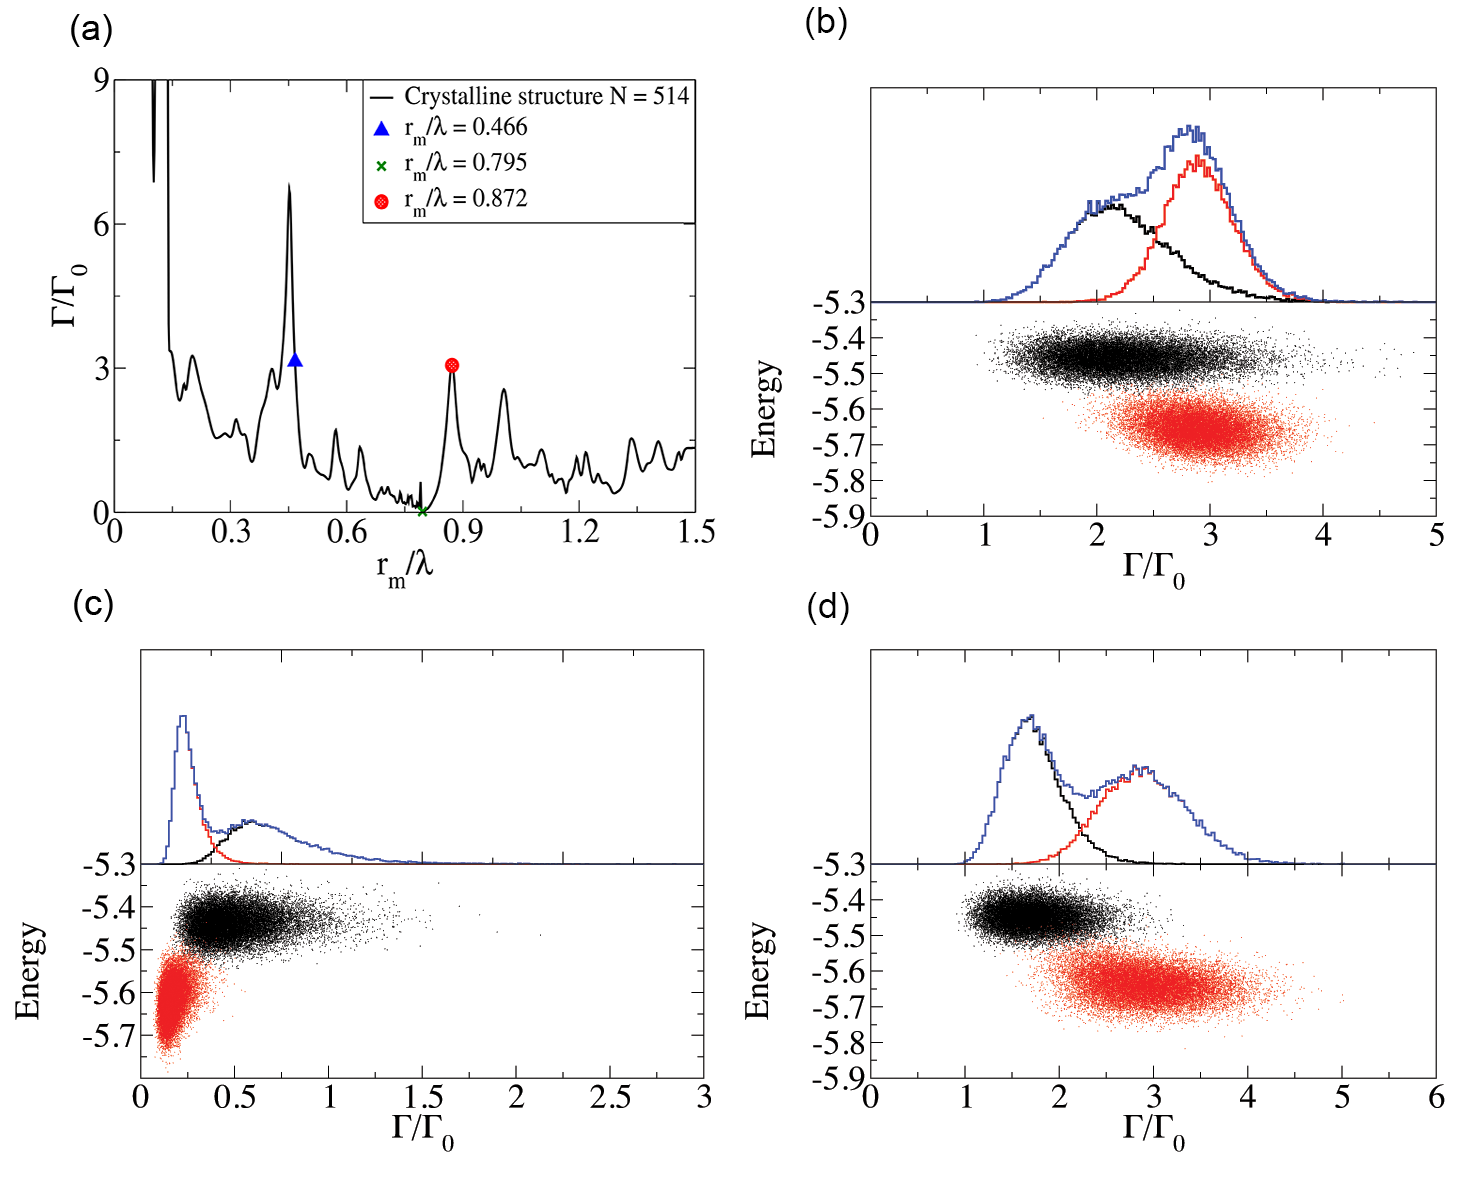
\includegraphics[width=12.5cm,angle=0]{chapter_8/figures/decay_rates.png}
\par\end{centering}
\caption{\label{fig:figm} (a) Normalized decay rates spectrum of a single emitter
placed at the center of a FCC cluster. \\
Energy-decay rate sampling at the switching region ($T\simeq0.53$, lower panels) for different ratios $r_{m}/\lambda$: (b) $r_{m}/\lambda=0.466$; (c) $r_{m}/\lambda=0.795$; (d) $r_{m}/\lambda=0.872$. Marked with symbols in (a). In the upper panels the corresponding normalized decay rates distributions are shown: red histograms correspond to the solid phase, black ones to liquid phase, and blues ones to total measured decay rates (sum of both liquid and solid distributions).}
\end{figure}

%\begin{figure}[h]
%\begin{centering}
%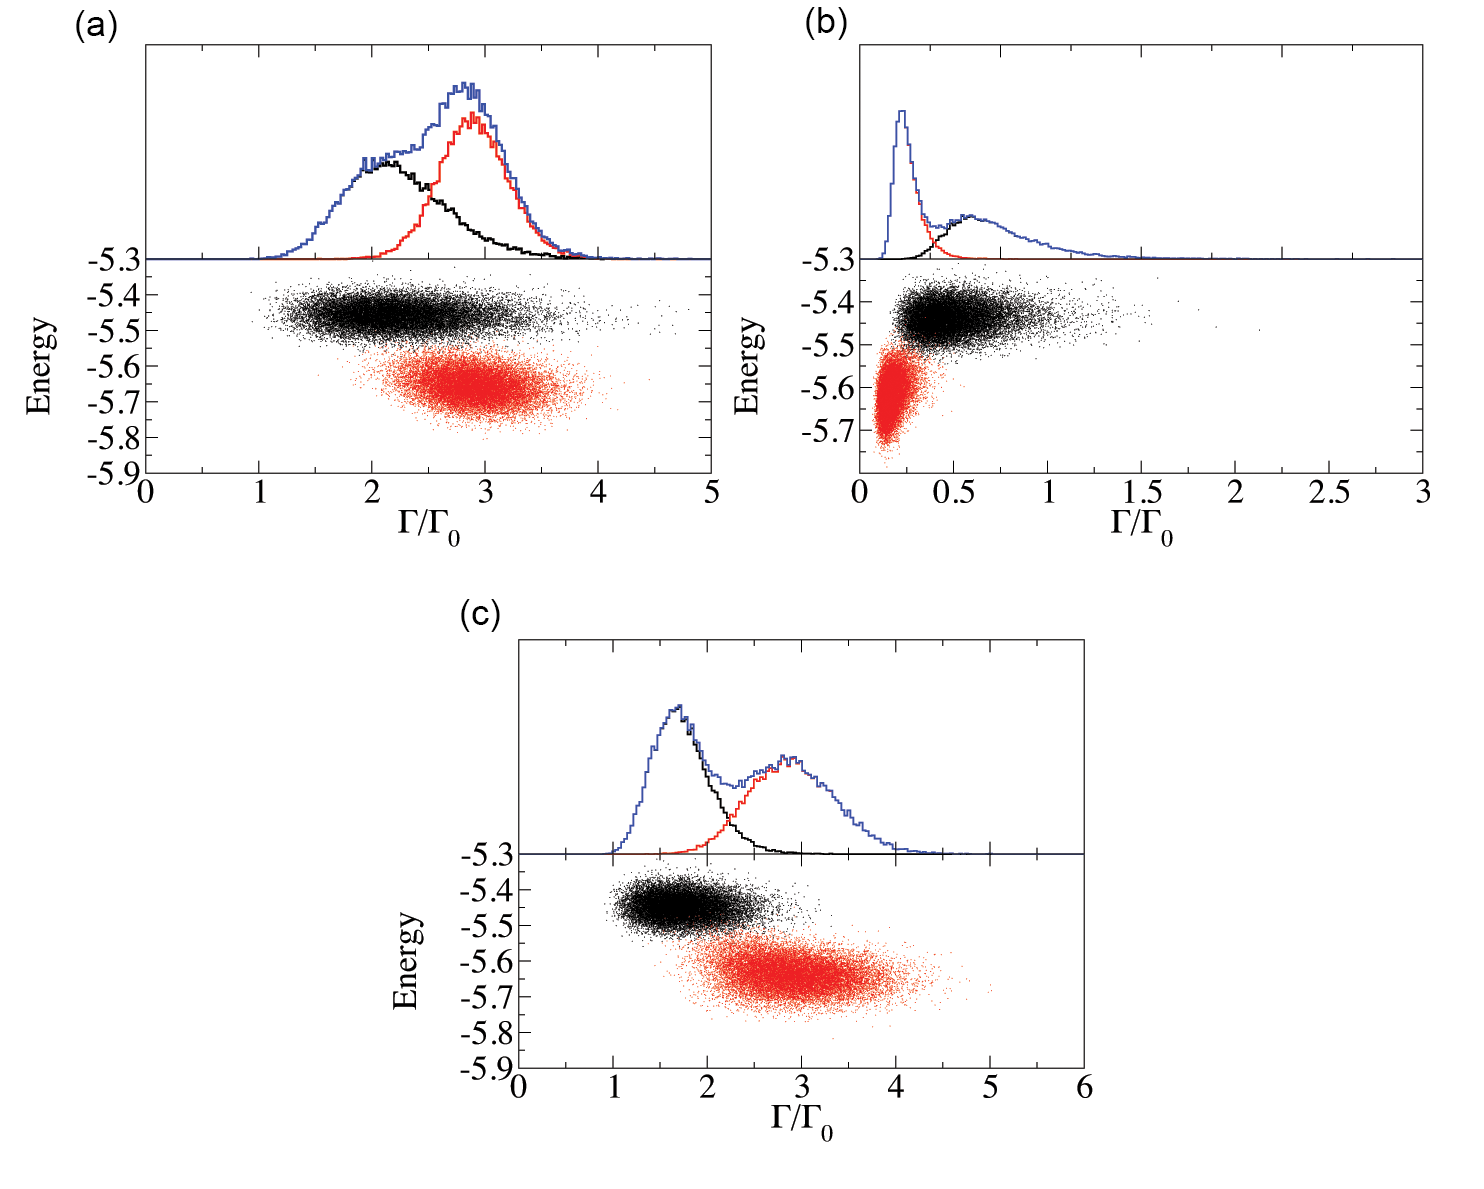
\includegraphics[width=13cm]{chapter_8/figures/image_4.png}
%\par\end{centering}
%\caption{\label{fig:fig4}Energy-decay rate sampling at the switching region
%($T\simeq0.53$, lower panels) for different ratios
%$r_{m}/\lambda$: (a) $r_{m}/\lambda=0.466$; (b) $r_{m}/\lambda=0.795$;
%(c) $r_{m}/\lambda=0.872$. Marked with symbols in Fig. \ref{fig:fig3}). In the upper panels the corresponding normalized decay rates distributions are shown: black histograms correspond to the solid phase, red ones to liquid phase, and blues ones to total measured decay rates (sum of both liquid and solid distributions).}
%\end{figure}

The statistical distributions of energy in Fig. (\ref{fig:figm})(b-d) obviously do not depend on the chosen ratios of $r_{m}/\lambda$. Although the distributions of decay rates show large variations with $r_{m}/\lambda$, there is a common feature among all the decay rate distributions: the lower energetic levels (solid phase, red distributions) are different from the higher energetic levels (liquid phase, black distributions), as seen in the upper panels. In particular its average values and fluctuations are appreciably different.\\
Measuring in a real experiment both internal energy of the interacting scatterers and the decay rate of the single emitter is far from being trivial. We might realise an experiment in which only emission lifetimes are measured for a single emitter. In this case, the only accessible quantity would be the decay rate irrespective of the value of the internal energy of the system. For the system under study, this would correspond to the added distributions plotted in blue in the upper panels of fig. (\ref{fig:figm})(b-d). Even in this case, the statistical distribution of decay rates show a signature of phase switching: Irrespective of the value of $r_{m}/\lambda$, the distributions are bimodal. \\
As mentioned, regarding the structural properties of the system in both phases in the phase-switching regime, the radial distribution functions are indistinguishable among phases, being the self-diffusion constant and the energy the only magnitudes clearly indicating that the system is in this dynamical regime. In order to clarify the origin
of the statistical signatures of phase switching in single emitter decay rates, we turn to analyse the radial distribution function of scatterers around the emitter. Our guess is that, if the diffusion of scatterers is dramatically different from one phase to the other, probably this fact has an impact on the radial distribution function and, in turn, on the statistics of decay rates.\\
In Fig. (\ref{fig:chap8_fig5}) we present the radial distribution functions (RDF) at different temperature regimes. Like before, we are able to distinguish among phases in a single MC run at constant temperature. This allow us to obtain the RDF of scatterers surrounding the emitter at liquid or at solid phases in the switching regime. The RDF is defined as the probability of finding a particle at a distance $r$ from the emitter $P\left(r\right)$ normalized by the probability in absence of any correlation $\left(\propto r^2\right)$.\\
We plot the RDF at a temperature $T \simeq 0.53$ for both the solid and the liquid  phases. Despite the fact that the two RDF among scatterers are indistinguishable, shown in Fig. (\ref{fig:chap7_Radial-distribution-function}) of the previous chapter, the RDF between scatterers and emitter is quite different. The RDF corresponding to the solid phase shows a richer structure with more pronounced peaks, while the one corresponding to the liquid phase is smoother and with wider peaks.

If we compare the RDF of the liquid phase at $T \simeq 0.53$ with the RDF
found at $T=1$, a temperature at which the system does not show phase switching and hence we call it as ''pure liquid phase'', we see that both distributions roughly coincide as shown in Fig. (\ref{fig:chap8_fig5})(b). Correspondingly, in Fig. (\ref{fig:chap8_fig5})(c) we compare the RDF of the solid phase in the phase switching regime with the RDF at $T=0.4$, which corresponds to a ''pure solid phase'' at a temperature just below the onset of the phase switching regime. We see that the RDF of the pure solid phase is also analogous to the one at the phase switching regime. In this case the correspondence is not as exact as in the liquid phase case, probably due to a stronger dependence of the RDF on the temperature for the solid phase.

\begin{figure}[H]
\begin{centering}
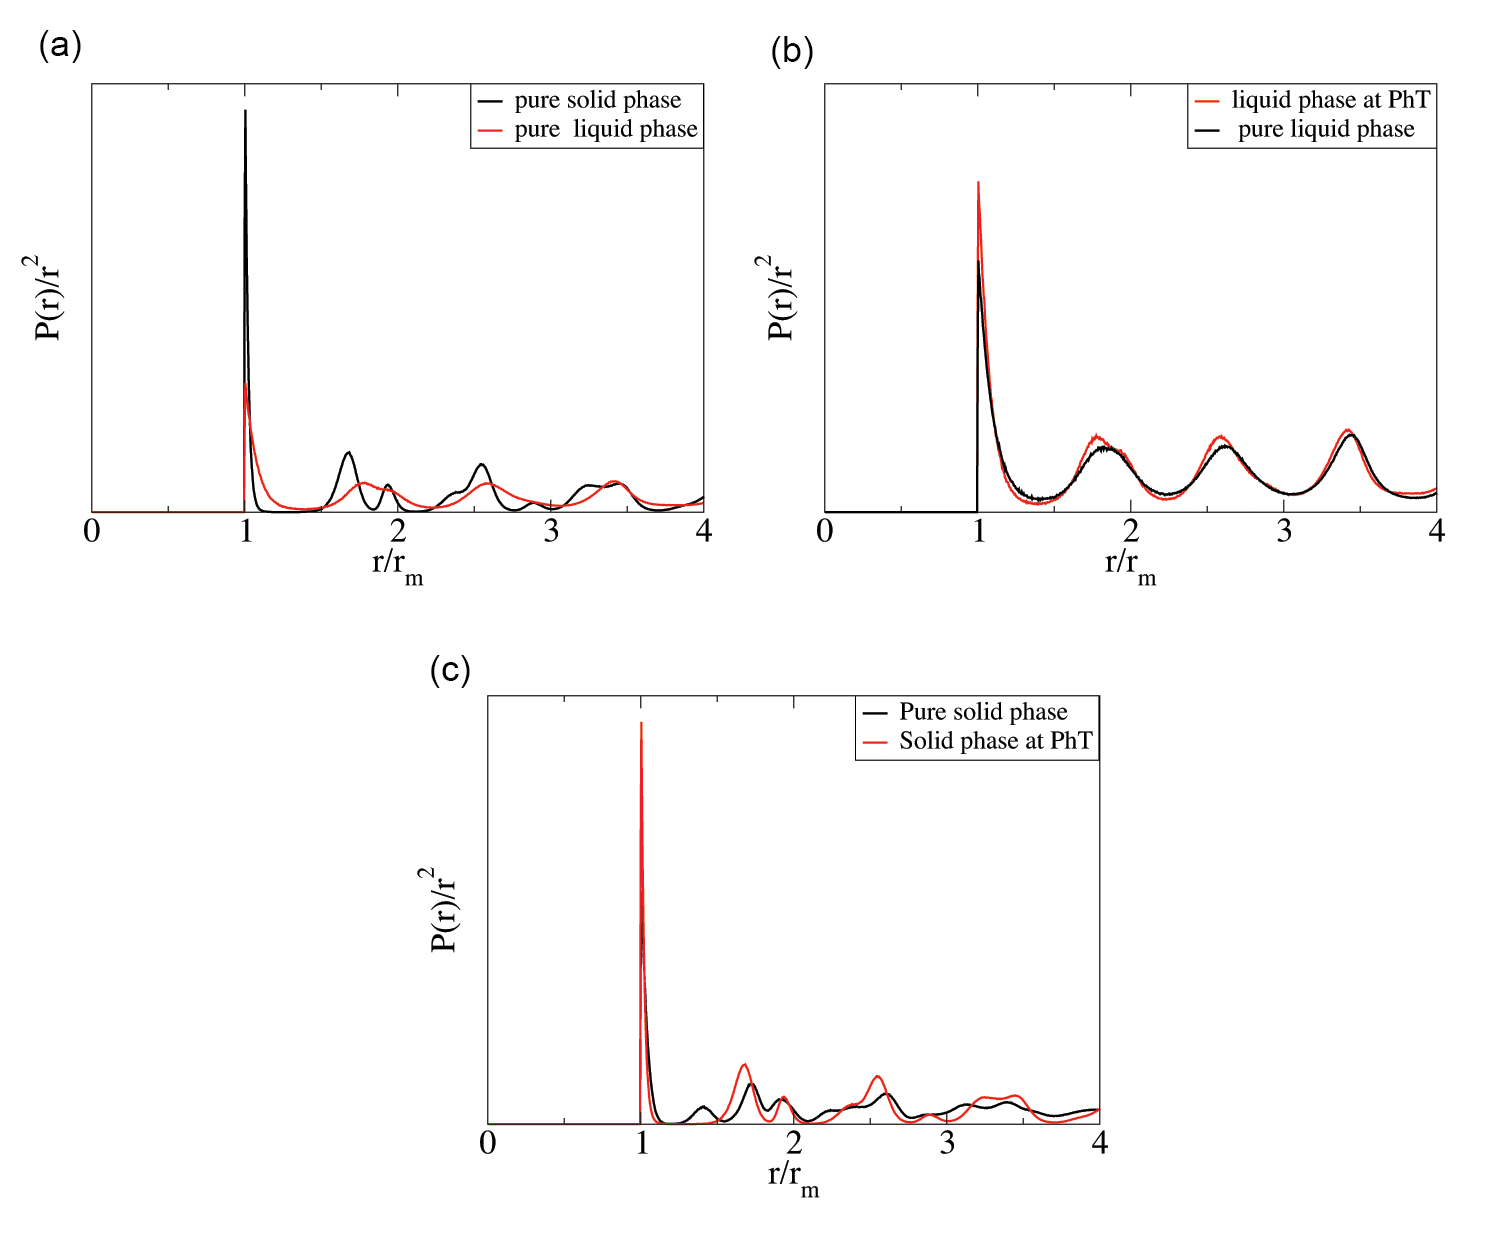
\includegraphics[width=12.5cm]{chapter_8/figures/RDF.png}
\par\end{centering}
\caption{\label{fig:chap8_fig5} Radial distribution function for scatterers surrounding the emitter placed at the center of the distribution in the phase-switching region. Liquid and solid phases are discriminated. (a) comparison of RDFs for the pure solid phase ($T =0.4$) with one in a pure liquid phase ($T=1$); (b) comparison of RDFs for the liquid phase ($T \simeq 0.53$) in the phase switching region with one in a pure liquid phase ($T=1$); (c) comparison of RDFs for the solid phase ($T \simeq 0.53$) in the phase switching region with one in a pure solid phase ($T=0.4$).}
\end{figure}



The above results suggest a relation between different decay rate statistics and structural properties of the system. The differences in the RDF can clearly be associated to the different nature of the phases, liquid or solid, as shown in the previous paragraphs. The different RDF might be the result of the large differences in the self-diffusion constant on the liquid and solid phases: in the liquid phase the scatterers can be arranged around the scatterers different ways as compared to the solid phase. It must to be noticed that the RDF among scatterers is indistinguishable and it is only the distribution of scatterers around a pinned emitter what shows differences among phases. \\
We suggest then that the above results are consistent with relatively subtle differences in the light scattering with scatterers which lie relatively close to the emitter, at distances comparable to a few wavelengths. In fact, as can be observed in Fig. (\ref{fig:chap8_fig5})(a), the RDFs for liquid and solid phases become more similar as the distance to the emitter increases, hence scatterers further apart than a few $r_{m}$ should not contribute to the differences in the decay rate statistics.

\section{Conclusion\label{sec:chap8_conclusion}}

In this chapter we have studied a model system of interacting light scatterers that present a solid-liquid phase transition. In the case where the system is relatively small (few hundreds of scatterers) and strongly confined, the system can enter in a phase switching regime where it switches among phases in its entirety in a certain range of temperatures. We have shown that, due to the fact that inter-particle RDF is indistinguishable between both phases, light scattering experiments are not able to discriminate if the system is in the switching regime. \\
Surprisingly, we find that single emitter decay-rate statistics experiments might, in principle, present strong signatures of the phase switching regime if performed in an appropriate way, in particular with low diffusivity emitters. We attribute this behaviour to the difference in the RDF between scatterers and the emitter position which, in turn, might also be attributed to differences in the self-diffusion of scatterers between both phases.\\
%The system we have considered presents an illustration of one deep difference between light scattering and light emission. 
The behaviour of this system clearly illustrates the fundamental differences between light emission statistics, (\textit{e.g.} $C_{0}$ correlations and LDOS fluctuations) and transport statistics, the former providing much more information about the statistical properties of the microstructure of the system.\\
Apart from the fundamental implications of this effect, it might be used as a tool for monitoring subtle thermodynamical behaviours of complex systems at sizes comparable with the wavelength of the light source employed in the experiment.\\
%The behaviour of this system clearly illustrates the fundamental differences between light emission statistics, (\textit{e.g.} $C_{0}$ correlations and LDOS fluctuations) and transport statistics, the former providing much more information about the statistical properties of the microstructure of the system.















